\documentclass[UTF8]{ctexart} 
\usepackage{amsmath} 
\usepackage{graphicx}
\usepackage{pythonhighlight}
\usepackage{indentfirst}
\usepackage{amsfonts}
\usepackage{graphicx}
\usepackage{subfig}

% \usepackage{algorithm}
\usepackage[]{algorithm2e}
\begin{document} 

\title{Homework 5}
\author{Ji Jiabao}
\maketitle

\subsection*{Exer.1}
    Denote the original r-s-flow and s-t-flow as $f_{rs}$ and $f_{st}$ respectively,
    we use them to construct a new r-t-flow $f_{rt}$, thus prove the transitivity of flow.
    
    Let 
    $$ f_{rt} = V \times V \rightarrow \mathbb{R} = \left\{
        \begin{aligned}
        f_{rs}(u, v) & & f_{rs}(u,v) \neq 0 \\
        f_{st}(u, v) & & f_{st}(u, v) \neq 0 \\
        0 & & otherwise\\
        \end{aligned}
        \right.
    $$
    Here $V$ is the set of all vertices.

    We just need to prove $f_{rt}$ is a flow.
    \begin{itemize}
        \item Capacity constraint: \\
            Case1: $f_{rs}(u,v) \neq 0$, then $f_{rt}(u,v) = f_{rs}(u,v) \le c(u,v)$\\
            Case2: $f_{st}(u,v) \neq 0$, then $f_{rt}(u,v) = f_{st}(u,v) \le c(u,v)$\\
            Case3: Otherwise, $f_{rt}(u,v) = 0 \le c(u,v)$, since $c(u,v) \ge 0$\\
        \item Skew symmetry: \\
            Case1: $f_{rs}(u,v) \neq 0$, then $f_{rt}(u,v) = f_{rs}(u,v) = -f_{rs}(v,u) = -f_{rt}(v,u)$\\
            Case2: $f_{st}(u,v) \neq 0$, then $f_{rt}(u,v) = f_{st}(u,v) = -f_{st}(v,u) = -f_{rt}(v,u)$\\
            Case3: Otherwise, $f_{rs}(u,v) = 0, f_{st}(u,v) = 0 \Rightarrow f_{rt}(u,v) = 0$\\
                                $f_{rs}(v, u) = -f_{rs}(u,v) = 0, f_{st}(v,u) = 0 \Rightarrow f_{rt}(v,u) = 0$\\
                                $f_{rt}(u,v) = 0 = -f_{rt}(v,u))$\\
        \item Flow conservation: \\
            For all $u \in V / \{r,t\}$,
            $$
            \begin{aligned}
                \sum_{v \in V}f_{rt}(u, v) &=\sum_{v \in V, f_{rs}(u,v) > 0}f_{rt}(u,v) + \sum_{v \in V, f_{rs}(u,v) > 0}f_{rt}(u,v) + \sum 0\\
                & = \sum f_{rs}(u,v) + \sum f_{st}(u,v) + 0\\
                & = 0 + 0 + 0\\
                & = 0\\
            \end{aligned}
            $$
    \end{itemize}

\subsection*{Exer.2}
    First we prove the easy part, these two cases will not occur simultaneously.Prove it by contradiction.

    Suppose both cases are true simultaneously, then there are $k$ vertex disjoint paths $p_1, ..., p_k$ from $s$ to $t$.
    and there exists $v_1, ..., v_{k - 1}$ such that $G - \{ v_1, ...,v_{k - 1}\}$ contains no 
    s-t-path. 
    
    For any $v_1, ..., v_{k - 1}$, the can take place in at most $k - 1$ paths in $p_1,...,p_k$ since $p_1, ..., p_k$ are
    disjoint vertex paths. Then we know there must be at least one path from $p_1,..,p_k$ left, which connects $s$ and $t$,
    leading to a contradiction.


    Next we prove that one of them must occur.

    The second case is obvious since we can just remove all vertices except $s, t$ from the $V$, then obviously there're no
    s-t-path now.

    For the first case, we construct such network-graph. Edges connecting with $s, t$ are assigned with $\infty$ capacity so
    that it will not affect the inner flow. All other edges are assigned with capacity $1$.

    \begin{figure}[h]
        \centering
        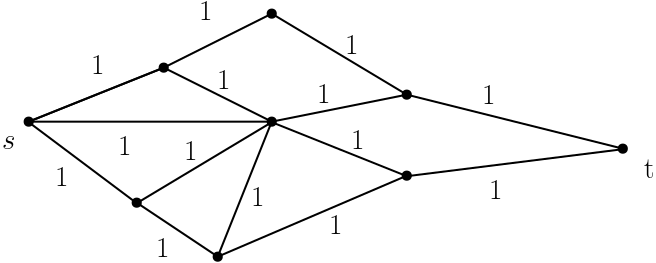
\includegraphics[scale=0.3]{figs/123.png}
        \caption{network}
    \end{figure}

    In such a network, the value of a flow is the number of vertex disjoint paths in such a flow. 
    Since the capacity of each edge is $1$, we can know for sure that no two s-t-path cross with each other,
    otherwise there must be a vertex with units bigger than 1. Based on that, we see $k$, the value of a flow 
    is the number of paths in it. Thus leading to $k$ disjoint paths.

\end{document}

